\documentclass[aspectratio=43]{beamer}

\usepackage[utf8]{inputenc}

\usepackage{color}
\usepackage{listings}
\usepackage{tikz}
\usepackage{hyperref}

\usetheme{Rochester}
\usecolortheme{beaver}

\addtobeamertemplate{navigation symbols}{}{%
    \usebeamerfont{footline}%
    \usebeamercolor[fg]{footline}%
    \hspace{1em}%
    \insertframenumber/\inserttotalframenumber
}

\lstloadlanguages{C++}
    \lstset{%
        language={C++},
        basicstyle=\ttfamily,
        keywordstyle=\color{blue},
        showstringspaces=false,
        escapechar={§},
        escapeinside=||
    }

\newif\iftransitions
 \transitionstrue


\newif\iffast
% \fasttrue

\title{Introduction to C++}
%\subtitle{Lua for C++ Programmers}
\author{Andreas Weis}
%\institute{BMW AG}
\date{GameCamp Munich, May 5, 2018}
\titlegraphic{
\includegraphics[height=.25\textheight]{resources/gcmuc_header_2018.png}}


\begin{document}

\frame{\titlepage}


\begin{frame}
  \frametitle{What is C++}
  \pause
  \begin{itemize}[<+->]
  \item Multi-paradigm
  \item Portable
  \item Largely backwards compatible with C
  \item Leave no room for a lower-level language
  \item You don't pay for what you don't use
  \end{itemize}
\end{frame}


\begin{frame}
  \frametitle{History of C++}
  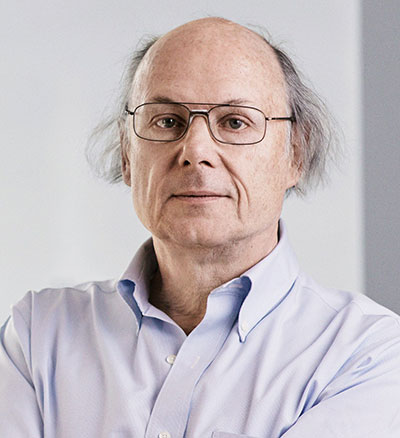
\includegraphics[height=.25\textheight]{resources/bjarne.jpg} \uncover<2->{
\includegraphics[height=.25\textheight]{resources/iso_logo.png}}
  \begin{itemize}[<+->]
  \item 1980s: Implemented by Bjarne Stroustrup at Bell Labs
  \item 1990s: Handed over to ISO for standardization (C++98)
  \item 2000s: ...
  \item 2010s: C++ Renaissance (C++11/14/17/20)
  \end{itemize}
  \uncover<4->{
\includegraphics[height=.25\textheight]{resources/isocpp_logo.png}}
\end{frame}


\begin{frame}
  \frametitle{Why learn C++ today?}
  \pause
  Why not?
  \pause
  \begin{itemize}[<+->]
  \item Lots of baggage from the 1970s
  \item Bloated, complicated and confusing
  \item It's much harder to learn than most other languages
  \item It's much harder to \emph{use} than most other languages
  \end{itemize}
\end{frame}


\begin{frame}
  \frametitle{Why learn C++ today?}
  \pause
  \begin{itemize}[<+->]
  \item It's extremely powerful
  \item It's largely domain-agnostic
  \item The best libraries
  \item Tool support is amazing
  \item Does not keep you away from the nuts and bolts
  \item If you know C++, picking up any other language is easy
  \end{itemize}
\end{frame}

\begin{frame}
  \frametitle{Where to start?}
  The Toolbox
  \pause
  \begin{itemize}[<+->]
  \item Compilers: gcc, clang/LLVM, MSVC
  \item IDEs: Visual Studio Community, JetBrains CLion, QtCreator, Eclipse, XCode
  \item CMake
  \end{itemize}
\end{frame}

\begin{frame}
  \frametitle{Where to start?}
  Resources
  \pause
  \begin{itemize}[<+->]
  \item The definitive C++ Book List
    \href{https://stackoverflow.com/questions/388242/the-definitive-c-book-guide-and-list}{https://stackoverflow.com/questions/388242/the-definitive-c-book-guide-and-list}
    \item \href{http://en.cppreference.com/w/}{cppreference.com}
    \item \href{https://isocpp.org/}{isocpp.org}
  \end{itemize}
\end{frame}

\begin{frame}
  \frametitle{Where to start?}
  Meet people
  \pause
  \begin{itemize}[<+->]
  \item MUC++ - Munich C++ User Group \href{https://www.meetup.com/MUCplusplus/}{https://www.meetup.com/MUCplusplus/}
  \item C++ Slack, \#learn \href{https://cpplang.now.sh/}{https://cpplang.now.sh/}
  \item Conferences:
  \begin{itemize}
    \item Meeting C++, Berlin \href{https://meetingcpp.com/}{https://meetingcpp.com/}
    \item CppCon, Bellevue USA \href{https://cppcon.org/}{https://cppcon.org/}
    \item C++Now, Aspen USA \href{http://cppnow.org/}{http://cppnow.org/}
    \item ACCU, Bristol UK \href{https://www.accu.org/index.php/conferences}{https://www.accu.org/index.php/conferences}
    \item NDC, Oslo \href{https://ndcconferences.com/}{https://ndcconferences.com/}
    \item code::dive, Wroclaw Poland \href{http://codedive.pl/}{http://codedive.pl/}
  \end{itemize}
  \end{itemize}
\end{frame}

\begin{frame}
  \frametitle{Thanks for your attention.}
\end{frame}


\end{document}
